\documentclass[tikz,border=12pt]{standalone}
\usepackage[T1]{fontenc}
\usepackage{mathpazo}
\usepackage{amsmath,amssymb}
\usetikzlibrary{arrows.meta, positioning, calc, fit, decorations.pathreplacing}

\definecolor{stblue}{HTML}{7B97AD}
\definecolor{rwgold}{HTML}{B8995E}
\definecolor{sage}{HTML}{7A9A7E}
\definecolor{dkbrown}{HTML}{3D3530}
\definecolor{wmgray}{HTML}{7B7067}
\definecolor{cream}{HTML}{F9F6F0}
\definecolor{border}{HTML}{D4C9B8}
\definecolor{terracotta}{HTML}{C47A6A}
\definecolor{lavender}{HTML}{907EA0}

\begin{document}
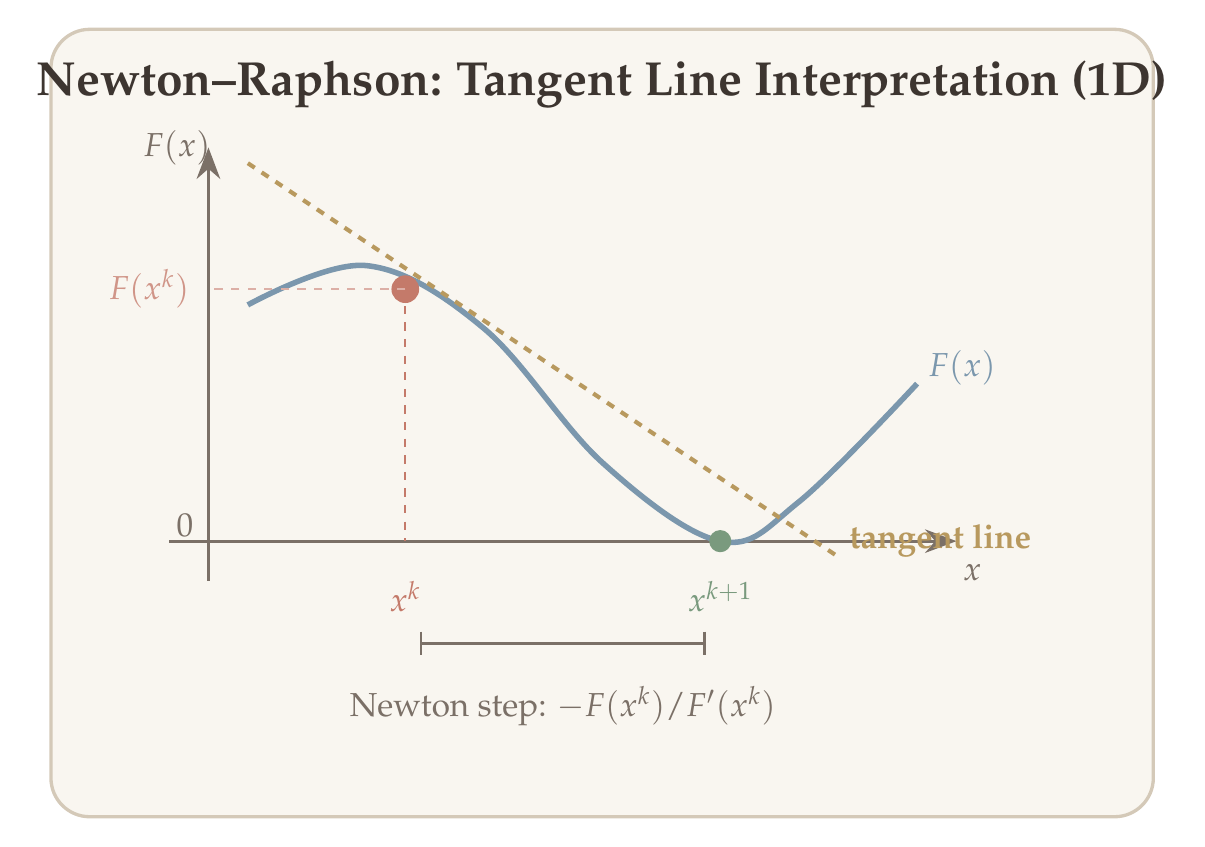
\begin{tikzpicture}[>={Stealth[length=4mm, width=3mm]}, line width=1.5pt]

% Background
\fill[cream, rounded corners=14pt] (-1.0,-3.0) rectangle (13.0,7.0);
\draw[border, line width=1.2pt, rounded corners=14pt] (-1.0,-3.0) rectangle (13.0,7.0);

% Title
\node[text=dkbrown, font=\LARGE\bfseries] at (6.0,6.3) {Newton--Raphson: Tangent Line Interpretation (1D)};

% Axes
\draw[wmgray, ->, line width=1pt] (0.5,0.5) -- (10.5,0.5);
\draw[wmgray, ->, line width=1pt] (1.0,0.0) -- (1.0,5.5);
\node[text=wmgray, font=\large] at (10.7,0.1) {$x$};
\node[text=wmgray, font=\large] at (0.6,5.5) {$F(x)$};
\node[text=wmgray, font=\large] at (0.7,0.7) {$0$};

% The curve F(x)
\draw[stblue, line width=2pt]
  plot[smooth, tension=0.6] coordinates {(1.5,3.5) (3.0,4.0) (4.5,3.2) (6.0,1.5) (7.5,0.5) (8.5,1.0) (10.0,2.5)};
\node[text=stblue, font=\large\bfseries, anchor=west] at (10.0,2.7) {$F(x)$};

% Current iterate x^k at approximately (3.5, 3.7) on the curve
\fill[terracotta] (3.5,3.7) circle (5pt);

% Vertical dashed line from x^k to axis
\draw[terracotta, dashed, line width=0.8pt] (3.5,3.7) -- (3.5,0.5);
\node[text=terracotta, font=\large\bfseries] at (3.5,-0.2) {$x^k$};

% Label F(x^k) on y-axis
\draw[terracotta!60, dashed, line width=0.6pt] (3.5,3.7) -- (1.0,3.7);
\node[text=terracotta!80, font=\large, anchor=east] at (0.9,3.7) {$F(x^k)$};

% Tangent line at (3.5, 3.7)
\draw[rwgold, dashed, line width=1.5pt] (1.5,5.3) -- (9.0,0.3);
\node[text=rwgold, font=\large\bfseries, anchor=west] at (9.0,0.5) {tangent line};

% x-intercept of tangent: x^{k+1}
\fill[sage] (7.5,0.5) circle (4pt);
\node[text=sage, font=\large\bfseries] at (7.5,-0.2) {$x^{k+1}$};

% Brace/bracket from x^k to x^{k+1} along axis
\draw[wmgray, line width=0.8pt] (3.7,-0.8) -- (7.3,-0.8);
\draw[wmgray, line width=0.8pt] (3.7,-0.65) -- (3.7,-0.95);
\draw[wmgray, line width=0.8pt] (7.3,-0.65) -- (7.3,-0.95);
\node[text=wmgray, font=\large] at (5.5,-1.6) {Newton step: $-F(x^k)/F'(x^k)$};

\end{tikzpicture}
\end{document}
